
%!TEX encoding = UTF-8 Unicode
%Einleitung/Schluss: Personenspezifische-
\documentclass[
    fontsize=12pt,
    headings=small,
    parskip=half,           % Ersetzt manuelles setzten von parskip/parindent.
    bibliography=totoc,
    numbers=noenddot,       % Entfernt den letzten Punkt der Kapitelnummern.
    open=any,               % Kapitel kann auf jeder Seite beginnen.
%   final                   % Entfernt alle todonotes und den Entwurfstempel.
    ]{scrreprt}

% ===================================Praeambel==================================

% Kodierung, Sprache, Patches {{{
\usepackage[T1]{fontenc}    % Ausgabekodierung; ermoeglicht Akzente und Umlaute
                            %  sowie korrekte Silbentrennung.
\usepackage[utf8]{inputenc} % Erlaub die direkte Eingabe spezieller Zeichen.
                            %  Utf8 muss die Eingabekodierung des Editors sein.
\usepackage[ngerman]{babel} % Deutsche Sprachanpassungen (z.B. Ueberschriften).
\usepackage{microtype}      % Optimale Randausrichtung und Skalierung.
\usepackage[
    autostyle,
    ]{csquotes}             % Korrekte Anfuehrungszeichen in der Literaturliste.
\usepackage{scrhack}        % Verhindert Warnungen mit aelteren Paketen.
% }}}

% Schriftarten {{{
\usepackage{mathptmx}       % Times. Package 'times.sty' is obsolete.
\usepackage[scaled=.92]{helvet}
\usepackage{courier}
\usepackage{placeins}
% }}}

% Biblatex {{{
% \usepackage[
%     style=alphabetic,
%     backend=biber,
%     backref=true
%     ]{biblatex}             % Biblatex mit alphabetischem Style und biber.
% \bibliography{Literatur.bib}% Dateiname der bib-Datei.
% }}}

% Dokument- und Texteinstellungen {{{
\usepackage[
    a4paper,
    margin=2.54cm,
    marginparwidth=2.0cm,
    footskip=1.0cm
    ]{geometry}             % Ersetzt 'a4wide'.
\clubpenalty=10000          % Keine Einzelzeile am Beginn eines Paragraphen
                            %  (Schusterjungen).
\widowpenalty=10000         % Keine Einzelzeile am Ende eines Paragraphen
\displaywidowpenalty=10000  %  (Hurenkinder).
\usepackage{floatrow}       % Zentriert alle Floats.
\usepackage{ifdraft}        % Ermoeglicht \ifoptionfinal{true}{false}
\pagestyle{plain}           % keine Kopfzeilen
% \sloppy                     % großzügige Formatierungsweise
\deffootnote{1em}{1em}{\thefootnotemark.\ } % Verbessert Layout mehrzeiliger Fußnoten

\makeatletter
\AtBeginDocument{%
    \hypersetup{%
        pdftitle = {\@title},
        pdfauthor  = \@author,
    }
}
\makeatother
% }}}

% Weitere Pakete {{{
\usepackage{verbatim}
\usepackage{graphicx}       % Einfuegen von Graphiken.
\usepackage{tabu}           % Einfuegen von Tabellen.
\usepackage{multirow}       % Tabellenzeilen zusammenfassen.
\usepackage{multicol}       % Tabellenspalten zusammenfassen.
\usepackage{booktabs}       % Schönere Tabellen (\toprule\midrule\bottomrule).
\usepackage[nocut]{thmbox}  % Theorembox bspw. fuer Angreifermodell.
\usepackage{amsmath}        % Erweiterte Handhabung mathematischer Formeln.
\usepackage{amssymb}        % Erweiterte mathematische Symbole.
\usepackage{rotating}
\usepackage[
    printonlyused
    ]{acronym}              % Abkuerzungsverzeichnis.
\usepackage[
    colorinlistoftodos,
    textsize=tiny,          % Notizen und TODOs - mit der todonotes.sty von
    \ifoptionfinal{disable}{}%  Benjamin Kellermann ist das Package "changebar"
    ]{todonotes}            %  bereits integriert.
\usepackage[
    breaklinks,
    hidelinks,
    pdfdisplaydoctitle,
    pdfpagemode = {UseOutlines},
    pdfpagelabels,
    ]{hyperref}             % Sprungmarken im PDF. Laed das URL Paket.
    \urlstyle{rm}           % Entfernt die Formattierung von URLs.
\usepackage{breakurl}
\def\UrlBreaks{\do\/\do-}
\usepackage{listings}       % Spezielle Umgebung für...
    \lstset{                %  ...Quelltextformatierung.
        language=[5.0]Lua,
        breaklines=true,
        breakatwhitespace=true,
        frame=L,
        captionpos=b,
        xleftmargin=6ex,
        tabsize=4,
        numbers=left,
        numberstyle=\tiny,
        basicstyle=\ttfamily\footnotesize,
        keywordstyle=\bfseries\color{green!50!black},
        commentstyle=\itshape\color{magenta!90!black},
        identifierstyle=\ttfamily,
        stringstyle=\color{orange!90!black},
        showstringspaces=false,
        }
% }}}

% ===================================Dokument===================================

\title{IT-Sicherheit und Schutz vor Malware im Automobil}
\author{Arne Beer, Stefan Grusche, Joshua Stock}
% \date{01.01.2015} % falls ein bestimmter Tag eingesetzt werden soll, einfach diese Zeile aktivieren

\begin{document}

\begin{titlepage}
\begin{center}\Large
    Universität Hamburg \par
    Fachbereich Informatik
    \vfill
    \makeatletter
    {\Large\textsf{\textbf{\@title}}\par}
    \makeatother
    \bigskip
    am Arbeitsbereich Sicherheit in Verteilten Systemen (SVS) \par
    \bigskip
    \makeatletter
    {\@author} \par
    \makeatother
    \bigskip
    \makeatletter
    {\@date}
    \makeatother
    \vfill
    \vfill
\end{center}
\end{titlepage}




\chapter*{Abstract}
In modernen Automobilen werden immer häufiger computergestützte Systeme integriert. Diese dienen hauptsächlich dem Zweck, die Sicherheit von Insassen und fremden Verkehrsteilnehmern zu verbessern, indem dem Fahrzeugführer zunehmend die Kontrolle aus der Hand genommen wird. Einhergehend mit dieser Integration erhalten jene Komponenten immer häufiger Zugriff auf elementare Bestandteile des Fahrzeugs, beispielsweise auf Lenkung und Bremsen. \par
Um das potentielle Sicherheitsrisiko, das (teil-)automatisiertes Fahren in Kombination mit einer üblicherweise hohen Vernetzung birgt, zu diskutieren, wurde zunächst der CAN-Bus als zentrale Netzkomponente untersucht. Anschließend wurde auf die verwundbarsten Teilsysteme eines vernetzten Automobils eingegangen, bevor die detaillierte Vorgehensweise einer Cyber-Attacke auf ein Fahrzeug dargestellt wurde. Abschließend wurden mögliche Maßnahmen, um vorhandene Sicherheitslücken zu schließen, aufgezeigt und diskutiert.

\tableofcontents

\chapter{Einleitung}
%Überarbeitete Fassung:
Mit dem Ziel das Sicherheitsrisiko im Straßenverkehr zu minimieren, wurden und werden zahlreiche computergestützte Systeme entwickelt. Einerseits greifen diese direkt in Notsituationen ein, um Fahrzeuginsassen sowie anderen Verkehrsteilnehmer ggf. das Leben zu retten (zum Beispiel durch automatisierte Notfallbremsungen). Andererseits können sie schon im Vorfeld das Eintreten derartiger Notsituationen zu verhindern versuchen (zum Beispiel Spurhalteassistenten). Angetrieben von der allgemeinen Digitalisierung unseres Alltags finden auch zunehmend komplexere Multimediasysteme Einzug in moderne Automobile. Diese integrieren neben typischen Unterhaltungsanwendungen heutzutage auch Navigationssysteme, Möglichkeiten für WLAN-Hotspots oder gar Einparkassistenten, die dem Nutzer vor allem einen höheren Komfort bieten sollen. Gerade derartige Assistenten benötigen oft direkten Zugriff auf sicherheitskritische Funktionen, wie Lenkung oder Bremsen, und nehmen dem Fahrer so die alleinige Kontrolle über das Fahrzeug. \par
Genannte Systeme verfügen in den meisten Fällen über verschiedene Kommunikationsarten. Nicht nur die Bereitstellung von Online-Multimediadiensten (zum Beispiel Musikstreaming), sondern auch der Austausch von Daten mit dem Hersteller verlangen eine digitale Verbindung zur Außenwelt. Da nicht nur Sicherheits-, sondern oft auch Multimediasysteme Zugriff auf fahrzeuginterne Netze zwischen kritischen Komponenten besitzen, existiert ein besonderes Schutzbedürfnis sämtlicher im Fahrzeug befindlicher Systeme. \par
Diese Arbeit dient dem Überblick über den aktuellen Forschungsstand im Bereich der automobilen Sicherheit, wobei der Fokus auf dem Komprimittieren von Fahrzeugen über integrierte Computersysteme liegt. Wir konzentrieren uns auf Angriffe, die ohne physische Verbindung zum Fahrzeug stattfinden und gegebenenfalls über große Distanzen ausgeführt werden können. \par
Einleitend werden wir uns mit den Grundlagen des sogenannten "`CAN-Busses"' beschäftigen. Wir erklären die Funktion des Busses und wie die Nachrichtenübertragung im Detail abläuft. Zusätzlich untersuchen wir die Sicherheit dieser Art des Nachrichtenaustauschs. Wir stellen eine Auswahl wichtiger Angriffsvektoren vor, die ein Angreifer, der nicht in physischem Kontakt zum Fahrzeug steht, nutzen kann, um ein Automobil zu komprimittieren und zeigen anhand von Forschungsergebnissen Miller und Valaseks \cite{MiV15}, dass diese auch außerhalb der Theorie von Bedeutung sind. In Anbetracht des aktuellen Sicherheitsstandes in der Automobilindustrie fassen wir abschließend verschiedene Vorschläge zur Verbesserung der IT-Sicherheit aus diversen Arbeiten zusammen.


%Ursprüngliche Fassung:
%In der heutigen Zeit befindet sich in jedem modernen Automobil eine hohe Anzahl fortgeschrittener technischer Systeme. Viele dieser Systeme sollten die Sicherheit der Insassen verbessern oder dem Fahrer assistieren, können durch enge Kopplung an sicherheitskritische Komponenten (Bremsen, Servolenkung, etc.) jedoch missbraucht werden um das Fahrzeug zu manipulieren.

%Ein hoher Grad an Vernetzung macht es immer leichter extern Zugriff auf das Auto zu erlangen. Daher rückt durch zunehmenenden Digitalisierung die Frage der Systemsicherheit immer mehr in den Vordergrund.

\chapter{Hauptteil}
\section{CAN-Bus}
\subsection{Funktion und Aufbau}
Die meisten IT-Sicherheitslücken in Fahrzeugen bauen auf Schwachstellen in der zentralen Kommunikationsschnittstelle eines Autos, dem sogenannten CAN-Bus, auf.\par
Der "`Controller Area Network"' Bus ist ein klassisches Binary Unit System, welches die meisten Systeme eines PKWs miteinander verbindet. Hierbei ist anzumerken, dass in vielen Autos mehrere CAN-Busse verbaut sind, welche unabhängig voneinander agieren können. Die an den CAN-Bus beziehungsweise die CAN-Busse gebundenen Systeme und Komponenten werden "`Electronic Control Units"' genannt, kurz ECUs\footnote{"`Electronic Control Units"'können Geräte verschiedenster Art sein und müssen keine Verbindungen zur Außenwelt aufweisen. ECUs sind entscheidende Bauteile eines Automobils und ihre korrekte Funktionsweise sind unverzichtbar für einen geregelten Betrieb. Beispiele für ECUs wären Parkassistenz-Systeme oder Lenkwinkelsensoren. Weitere Beispiele siehe Abb. 2.1}, eine spezielle Art von TCUs sind "`Telematic Control Units"'\footnote{"`Telematic Control Units"': Steuergeräte für Telematikdienste. Sind in der Regel direkt an den CAN-Bus angeschlossen und zeichnen sich häufig durch viele ausgehende Verbindungen aus (Bluetooth, Mobilfunk, GPS, etc.)}.\par
Die übliche Funktionsweise eines CAN-Busses lässt sich gut am Beispiel des Toyota Prius erklären \cite{MiV13}: ECUs kommunizieren untereinander über den Bus, wobei jedes gesendete Paket an jede andere ECU am selben Bus gesendet wird ("`Broadcast"'). Die ECUs selbst entscheiden anschließend anhand der Struktur der Pakete, ob die Informationen für sie bestimmt sind und verarbeiten diese, falls dies der Fall ist.\par

\FloatBarrier
\begin{figure}[h!]
	\centering
  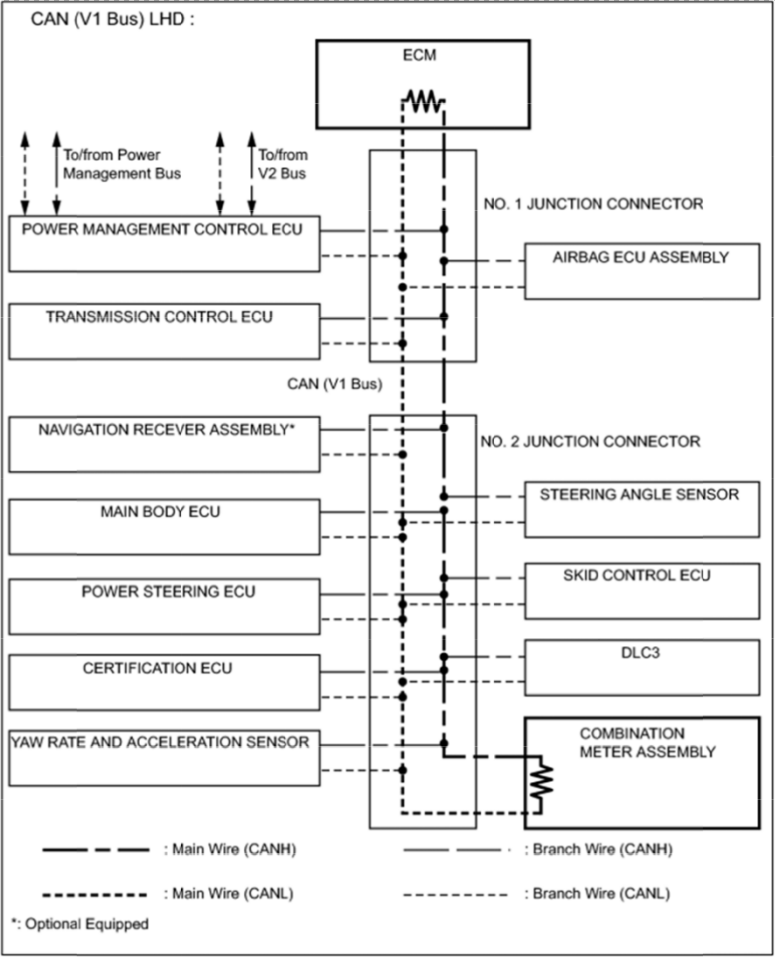
\includegraphics[width=0.7\textwidth,keepaspectratio]{pic/can-bus.png}
	\caption{Schematischer Aufbau eines CAN-Busses \cite{MiV13}.}
\end{figure}
\FloatBarrier
\newpage


Nachfolgend ein Beispiel für ein Paket, das auf einem CAN-Bus kommuniziert wird, in hexadezimaler Schreibweise:

\centerline{\texttt{00 B4 08 00 00 00 00 3C 18 C0 FF}}

Das Paket kann wie folgt interpretiert werden:
Die ersten 2 Byte, in obiger Schreibweise durch $00\;B4$ repräsentiert, definieren den Identifikator ('ID') der adressierten ECU. Die nachfolgenden 4 Bit definieren die Länge der nachfolgenden Nutzdaten, also der relevanten Daten oder dem Befehl. In diesem Falle sind es 8 Byte, also die Sequenz (00 00 00 00 3C 18 C0 FF).

Obiger Befehl ließe sich auch in folgender Schreibweise darstellen, auch wenn hierbei durch die fehlenden Byte Informationsverlust auftreten kann:

\centerline{\texttt{00 B4 04 3C 18 C0 FF}}

In diesem Paket wird lediglich eine Nutzdatenlänge von 4 Byte definiert. Um Nachrichtenintegrität sicherzustellen, wird häufig eine Prüfsumme erstellt. Diese wird üblicherweise als letztes Byte der Nutzdaten an das Paket gehängt und wird durch einen vom Hersteller definierten Algorithmus generiert.
Im Folgenden beispielhaft ein Befehl an das Geschwindigkeitstacho eines Ford Escape:
Die Addresse ist wie vorher $00\;B4$ mit einer Nutzdatenlänge von $08$. Die Nutzdaten strukturieren sich wie folgt:

\centerline{\texttt{AA BB 00 00 CC DD 00 00}}

$AA BB$ definiert die RPM, während $CC DD$ die Geschwindigkeit angibt. Die Werte werden nach folgenden Formeln berechnet:

\[\text{Speed} (mph) = 0.0065 \cdot (CC DD) - 67\]
\[RPM = 0.25 \cdot (AA BB) - 24\]

Dementsprechend würde ein Befehl mit ca. 100km/h und 2000RPM folgendermaßen aussehen:

\centerline{\texttt{1F 40 00 4E BC 00 00}}

Der komplette Befehl hätte die Form:

\centerline{\texttt{00 B4 08 1F 40 00 4E BC 00 00}}

Nehmen wir an, dass noch eine Prüfsumme angefügt wird, nach der Formel:

\[\text{Checksum} = (IDH + IDL + Len + Sum(\text{Data}[0]\text{ – }\text{Data}[Len-2])) \& 0xFF \]

Dementsprechend ist wäre das letzte Byte $CC$:

\centerline{\texttt{00 B4 08 1F 40 00 4E BC 00 CC}}

Der simple Aufbau der Pakete ist jedoch nur einer der Gründe, weshalb Angriffe auf den CAN-Bus vergleichsweise einfach sind.

\subsection{Sicherheit}
Wie bereits erwähnt, stellt die Kommunikation über den CAN-Bus das größte Sicherheitsproblem dar: Bei den meisten Autos verläuft diese vollkommen unverschlüsselt. Außerdem kommunizieren die ECUs ohne jegliche Authentifizierung. Deshalb können schadhafte Pakete auf den Bus gelegt werden und im Regelfall akzeptiert und verarbeitet es die betroffene ECU problemlos.\par
Ferner sind die Protokolle und Programmierschnittstellen ("`APIs"'), mit denen die ECUs kommunizieren, nicht öffentlich einsehbar und nur dem jeweiligen Hersteller bekannt. Zwar erschwert dies den Entwurf valider Pakete, allerdings kann ein Angreifer durch den Broadcast-Verkehr der Pakete auf dem CAN-Bus beliebig viele ebensolcher ohne Probleme für eine spätere Analyse mitschneiden.
Selbstverständlich wird dabei Zugriff auf den Bus selbst benötigt, die Analyse kann aber zum Beispiel auch an einem baugleichen Modell geschehen, welches der Angreifer besitzt oder mietet. Da der abgehörte Verkehr auf dem Bus unverschlüsselt ist, kann der Mitschnitt nun benutzt werden, um die API der ECUs zu rekonstruieren: Hierfür muss lediglich nach Mustern im Paketstrom gesucht werden, welche in Abhängigkeit zum Zustand des Autos stehen. Durch dieses Verfahren wurde beispielsweise die oben gezeigte API des Geschwindigkeitstachos rekonstruiert.

Durch das Senden und Empfangen Aller an Alle entsteht ein weiteres Problem. Mit jedem Gerät, welches an dem Bus hängt, wird ein neuer Angriffsvektor bereitgestellt.
Solange ein Angreifer physikalischen Zugriff auf den Bus hat, kann er also einen eigenen Empfänger am Bus befestigen oder die Firmware vorhandener ECUs manipulieren.
Durch die zunehmende Vernetzung des Automobils oder technisch beabsichtigte Bequemlichkeiten wie Firmware-Updates per CD/USB oder gar Funk/Internet, steigt die Kompromittierbarkeit von an dem CAN-Bus befindlichen Geräten zunehmend.

%Dies sind alles Probleme, welche mit einer Verschlüsselung und einem gut implementieren Authorisierungssystem hätten vermieden werden können. --> in Schlussteil

\section{Ausgewählte Angriffsvektoren}
Nicht alle Systeme, TCUs oder ECUs, die über den CAN-Bus kommunizieren, sind als Angriffsvektor geeignet. Entscheidend für einen Angriff ohne physischen Zugriff auf den Bus oder die Systeme selbst ist eine von außen erreichbare Verbindung. Neben vielen Geräten mit eingeschränkter Möglichkeit des unerlaubten Fremdzugriffes taten sich die folgenden drei Vektoren als besonders schwerwiegende Sicherheitslücken auf:

\subsection{Bluetooth}
%Joshua
Eine Bluetooth-Schnittstelle zählt mittlerweile zu der Standardausstattung eines modernen Autos. Ihre Hauptfunktion ist meist die Verbindung eines Mobiltelefons zum Media-System des Autos, um beispielsweise Anrufe über eine integrierte Freisprecheinrichtung entgegenzunehmen, aber auch, um Anrufe aus dem Auto über das Mobiltelefon zu starten oder Musik vom Mobiltelefon direkt über das Mediasystem des Autos wiederzugeben.
In dem PKW, den Checkoway et al. in \cite{CMK11} betrachten, befindet sich das Bluetooth Modul in der Telematik-Einheit. Checkoway et al. konnten durch Reverse-Engineering das Unix-ähnliche Betriebssystem analysieren, inklusive der Bluetooth-Stack-Implementation. Den Forschern gelang es wegen Sicherheitslücken in ebendieser Implementation, einen Kommandozeileninterpreter ("`Shell"') auf der Telematik-Einheit zu öffnen. \par
Sie unterscheiden zwischen zwei Angriffsmöglichkeiten: Zum einen werden \textit{indirekte} drahtlose Kurzstrecken-Attacken aufgeführt, bei denen ein bereits über Bluetooth mit der Telematik-Einheit gekoppeltes, beliebiges Android- oder iOS-Smartphone benötigt wird, zum anderen beschreiben sie \textit{direkte} drahtlose Kurzstrecken-Attacken. Für letztere muss die MAC-Adresse des Bluetooth-Moduls im Auto bekannt sein, diese kann allerdings mit wenig Aufwand durch verschiedene "`Sniffing"'-Software herausgefunden werden. Um nun eine Bluetooth-Kopplung zwischen Automobil und Angreifer zu erzwingen, muss lediglich eine PIN, die sich erst nach Neustart des PKWs ändert, herausgefunden werden. Auch diese stellte kein großes Hindernis dar, mittels Brute-Force-Methode gelang es den Forschern teilweise innheralb von 15 Minuten, sich ohne jede Benutzerinteraktion mit der Telematik-Einheit des Autos zu verbinden und die Bluetooth-Sicherheitslücken auszunutzen.\par
Miller und Valasek, die sich in \cite{MiV14} mit dem 2010 Ford Escape beschäftigten, konnten zwar keine Möglichkeit finden, ein Gerät ohne Benutzer-Interaktion mit dem Auto zu koppeln, sehen den Bluetooth Stack jedoch trotzdem durch seine Größe als "`eine der größten und machbarsten Angriffsflächen eines modernen Automobils"'.
% Quellen:
% cars-usenixsec2011 S. 8f, 12, 13, 14
% remote attack surfaces.pdf S. 15f, 90f
%NICHT BENÖTIGT Remote Car Hacking.pdf S. 16, 33

\subsection{Mobilfunk}
%Ich denke, dazu können wir auch kurz was sagen. Zum Beispiel usenixsec2011 "Long-range wireless channels: Cellular" ab S.9 als Quelle \j
Eine weitere ausgehende Verbindung der Telematikeinheit ist oftmals der Mobilfunk. Durch ein eingebautes 3G-Modem kann das Automobil so mit dem Internet verbunden sein, oder im Falle eines schweren Unfalls selbständig eine SMS an Rettungskräfte senden.\par
Über die Telematikeinheit können jedoch auch Kommandos übertragen werden. Durch das Mitschneiden des 3G-Verkehrs gelang es den Autoren von \cite{CMK11}, Teile des verwendeten Protokolls zu rekonstruieren. %Die Übertragung fand bei ca. 700Hz statt durch Frequency-shift keying (FSK), welche es erlaubt Daten durch Frequenzverschiebung eines Signals zu übertragen.
Durch Umschalten der Telematikeinheit-Software in den Debug-Modus konnten sich die Forscher alle ein- und ausgehenden Daten in Bitform anzeigen lassen. In Kombination mit den aufgezeichneten Daten war es ihnen möglich, die Paketstrukturen zu rekonstruieren. Die Software des Systems war darauf eingestellt, dass empfangene Pakete niemals größer als 100 Byte sind. Diese Sicherheitslücke machten sich die Forscher zunutze, um ein größeres Paket einzuschleusen, welches zu einem Buffer-Overflow führte. Dadurch wurde schädlicher Code in den Speicher des Systems geschrieben, teilweise direkt auf den Callstack des Programms. Eine vorhandene Sicherheitsmaßnahme, die nach wenigen Sekunden eine Authentifizierung des Absenders verlangt, konnte durch einfache Simulation der Authentifzierung leicht umgangen werden.
%Um ein Schadprogramm von der Größe von 300 Byte einzuschleusen, würde die 3G Verbindung jedoch ca. 14 Sekunden benötigen. Nach ca. 12 Sekunden wird von der Telematikeinheit jedoch eine Authentifizierungssequenz erwartet, sonst wird die Verbindung unterbrochen. Die Sequenz wird jedoch mit einem Pseudozufallscode generiert, welcher auf steets mit einer speziellen Konstante geseeded wird.
%Ein Angreifer ist also in der Lage durch zuvor mitgeschnittene Antwort Pakete eine Authentifizierung zu simulieren. Außerdem existiert noch eine weitere Sicherheitslücke in der Geniererung der Authentification-Challenge, sodass mit spezieller Formatierung ca. jeder 256te Authentifizierungsversuch gelingt.

%Durch diese Sicherheitslücken in der Authentifizierung ist es nun möglich ein Schadprogramm durch einen Bufferoverflow in den Speichern der Telematikeinheit einzuschleusen. So wurde zum Beispiel ein Befehl eingespielt, welcher zusätzliche Malware von einer per 3G im Internet erreichbaren Adresse herunterlädt und diese ausführt.

\subsection{Nachrüstbare TCUs}
Zusätzlich zu den unterschiedlichen Medien- und Diagnosesystemen, die bereits durch den Hersteller in die Fahrzeuge integriert sind, gibt es verschiedenste nachrüstbare Gerätschaften, die dazu dienen können, den Funktionsumfang eines Fahrzeugs zu erweitern (fortgeschrittene Medienanwendungen etc.) oder dem Fahrzeughalter detaillierte Informationen über den Zustand des Autos zu geben. Besonders interessant ist hierbei die Sparte der TCUs, \textit{Telematic Control Units}, die verschiedenste Funktionen und Anwendungszwecke besitzen können. Die meisten dieser TCUs verfügen dabei über einen GPS-Sensor, oft unterschiedliche Beschleunigungssensoren und eine Mobilfunk und/oder Internetanbindung, um entweder mit den externen Systemen des TCU-Herstellers kommunizieren zu können, sei es um zum Beispiel aufgezeichnete Daten zu Auswertungszwecken zu übertragen oder die eigene Soft- oder Firmware zu aktualisieren, oder um sich mit Endgeräten der Fahrzeuginsassen bzw. des Fahrzeughalters zu verbinden. \par
Ein prominentes Einsatzfeld nachgerüsteter TCUs ist die Aufzeichnung des Fahrverhaltens durch Versicherungen, die basierend auf den aufgezeichneten Daten ihre Beiträge berechnen. Eine in diesem Umfeld angewandte TCU ist zum Beispiel das Modul "`Snapshot"' der Firma Progressive. Andere TCUs (beispielsweise "`Automatic"' von Automatic Labs) zielen direkt darauf ab, das Fahrverhalten zu verbessern, indem sie über Smartphones der Fahrzeughalter in Echtzeit zum Beispiel Hinweise für eine motor- und benzinschonenderes Beschleunigungs- und Bremsverhalten geben. Häufig finden TCUs auch im Flottenmanagement Anwendung, wo sie zur Lokalisierung und Überwachung der Geschäftfahrzeuge dienen. "`Connect"' des Herstellers Delphi ist eine besonders funktionsreiche TCU, die neben bereits erwähnten Anwendungen wie der Lokalisierung auch detaillierte Informationen über die Gesundheit des Fahrzeugs ausgibt, für Eltern die Möglichkeit bietet, ihren Kindern einen Bereich zur Nutzung des Fahrzeugs festzulegen, als Schlüsselersatz zum Öffnen, Schließen und Starten des Autos dient und über 4G-Mobilfunk einen Internet-Hotspot für die Fahrzeuginsassen bereitstellen kann. \par
TCUs von Fremdherstellern werden üblicherweise direkt an den OBD-Port des Fahrzeugs angeschlossen und werden auf diese Weise direkt in das interne Netzwerk integriert, können im Allgemeinen Nachrichten vom CAN-Bus mitlesen und beinhalten oft auch selbst die Funktionalität, Nachrichten auf den CAN-Bus zu schreiben. Dies ist dabei die größte Gefahr einer nachgerüsteten TCU: eine oft umfangreiche Internet- oder Mobilfunkfähigkeit und dabei theoretisch uneingeschränkter Zugriff auf sicherheitskritische Systeme bietet Angreifern eine optimale Angriffsfläche, die bei einem erfolgreichen Eindringen von außen u.U. eine volle Kontrolle über das Fahrzeug bedeutet. \par
In \cite{FPK15} haben Foster et al. anhand einer TCU zur Fahrstilanalyse für Versicherungszwecke aufgezeigt, wie ein unsicherer Entwurf des Update-Protokolls letztendlich zur Übernahme des Geräts und damit zum Zugriff auf das Fahrzeug führen konnte. Im beschriebenen Fall waren sie in der Lage, nach Ausfindigmachen der Telefonnummer der TCU, die sie für Mobilfunkdienste besaß, mit einer einfachen SMS einen Update-Vorgang an einem beliebigen Server anzustoßen.
Aufgrund einer nicht vorhandenen Authentifizierung des Servers und einer ebenso fehlenden Signatur der Updates konnten beliebige eigene Dateien auf die TCU heruntergeladen werden und mit entsprechenden Befehlen ausgeführt werden. Im Endeffekt erlangten die Angreifer die Möglichkeit, sich mit Root-Berechtigungen in die TCU einzuwählen und erhielten somit freie Verfügung über das komplette System. Die Verbindung zum CAN-Bus bot dann an, selbst Nachrichten zu verschicken. In einer Proof-of-Concept-Attacke zeigten Foster et al. abschließend, dass sie u.a. in der Lage waren, die Scheibenwischer und einzelne Bremsen zu betätigen. \par
Fehler dieser Natur bei dem Entwurf derart sicherheitsrelevanter Systeme stellen also eine große Gefahr für den Fahrzeughalter dar. Diese wird noch dadurch verstärkt, dass der Fahrzeughersteller selbst nicht in der Lage ist, Fehler zu beheben. Da es sich um fremde Systeme handelt, muss hier der jeweilige Hersteller selbst aktiv werden und dafür sorgen, dass alle sich im Umlauf befindenen TCUs eventuelle Updates erhalten.

\section{Praxisbeispiel: 2014er Jeep Cherokee}

Im Folgenden stellen wir anhand der Forschungsergebnisse von Miller und Valasek aus \cite{MiV15} dar, wie ohne direkten Zugang verschiedene Funktionen auf diversen Systemen eines konkreten Fahrzeugs, in diesem Fall eines 2014er Jeep Cherokees, ausgeführt werden können und so eine direkte Gefahr für den Straßenverkehr geschaffen werden kann. \par
Der Jeep Cherokee besitzt einige Systeme, die für einen Angreifer von großem Interesse sein können. So ist u.a. ein adaptiver Tempomat, der von sich aus Fahrzeugbremsen auslöst, ein Kollisionswarnsystem, welches das Fahrzeug ebenfalls zu einem kompletten Halt bringen kann, ein Spurassistent, der, wenn auch minimal, in die Lenkung eingreifen kann, und einen Einparkassistenten, welcher wiederum komplette Kontrolle über das Lenkrad erhält, integriert. Des Weiteren ist ein Multimediasystem mit WLAN- und Mobilfunkverbindung eingebaut, welches gleichzeitig an beide vorhandenen CAN-Netzwerke im Auto angeschlossen ist. Aus genau diesem Grund ist dieses System das Hauptaugenmerk von Miller und Valaseks Arbeit, da über ein Kompromittieren der Medieneinrichtung potentiell die größte Kontrolle über das Auto erlangt werden kann. Die Autoren konzentrierten sich zunächst auf Schwächen der eingebauten Hotspot--Funktionalität; sofern der Fahrzeughalter ein Abonnement beim Hersteller abschließt, bietet das Fahrzeug an, einen WLAN-Hostpot für die Fahrzeuginsassen bereitzustellen. Das Netz an sich wies keine unüblichen Schwachstellen auf, Miller und Valasek konnten aber Schwächen bei der zufälligen Generierung der Netzpasswörter entdecken: Das Passwort wird stets durch eine Funktion berechnet, die auf dem Zeitpunkt des Aufrufens beruht. Dieser kann zusätzlich stark eingeschränkt werden, da sich das System, solange keine Uhrzeit über GPS oder Mobilfunk empfangen wurde, auf eine Standarduhrzeit einstellt. \par
Mit Verbindung zum WLAN-Netzwerk konnten Miller und Valasek mithilfe üblicher Netzwerkanalysetools diverse offene Ports identifizieren, die sich potentiell zum Ausführen von Angriffen anbieten. Insbesondere der Port 6667 erwies sich als interessant, da sich dahinter nicht, wie üblich, ein IRC-Server versteckte, sondern eine Variante von D-Bus über IP. D-Bus ist ein Framework, welches der Interprozesskommunikation dient: Es ermöglicht Prozessen, Funktionen an anderen Prozessen aufzurufen. Zusätzlich stellte sich heraus, dass sich ein Angreifer ohne Authentifizierung mit diesem System verbinden konnte. Mithilfe der D-Bus-Bibliotheken und eines Debugging-Tools konnten Miller und Valasek ohne Probleme aufrufbare Funktionen identifizieren, darunter eine, die vom Nutzer übergebene Shell-Kommandos ausführt: eine deutliche Sicherheitslücke und der attraktivste Angriffspunkt des Systems. \par
Über diese Lücke erwies es sich als trivial, Code auszuführen. Mit sehr simplen Skripten kann ein Angreifer nun unter anderem GPS-Daten auslesen, um den Standort des Fahrzeugs festzustellen, er kann die Geschwindigkeit der Lüfter, die Lautstärke (Beispielcode: siehe unten) und den Basspegel des Radios verändern, zusätzlich den Radiosender wechseln, bestimmen, was auf dem integrierten Display erscheint und eigene Bilder einspielen. \\
\begin{lstlisting}[caption=Beispielskript zum Ändern der Lautstärke.]
require "service"

params = {}
params.volume = tonumber(arg[1])
x=service.invoke("com.harman.service.AudioSettings", "setVolume", params)
\end{lstlisting}

Das Eindringen in ein WLAN-Netz, obwohl kein direkter physischer Zugriff zum Fahrzeug benötigt wird, kann nur aus begrenzter Entfernung, etwa 30m, erfolgen. Aus diesem Grund änderte sich nun der Fokus von Miller und Valasek auf die Mobilfunk-Fähigkeiten des Multimediasystems. Unter anderem für mobilen Internetzugang besitzt der Jeep eine 3G-Verbindung zum Netz eines Mobilfunkanbieters (Im konkreten Testfall handelte es sich um den amerikanischen Anbieter Sprint). Es konnte beobachtet werden, dass innerhalb des Netzes des Mobilfunkanbieters einerseits dem Fahrzeug stets eine IP-Adresse in einem von zwei Adressbereichen zugeordnet wird und andererseits auch in dieser Umgebung der Zugang zum D-Bus-System für fremde Geräte offen ist. Dies bedeutet, dass, sofern sich der Angreifer im Netz des gleichen Anbieters wie das Fahrzeug befindet, die zuvor beschrieben Attacken nicht nur in direkter Umgebung, sondern über das ganze Land (beziehungsweise der Reichweite des Netzbetreibers) ausgeführt werden können. Zudem konnten Miller und Valasek über IP-Analysen feststellen, dass diverse andere Fahrzeuge, die dasselbe Mediensystem integriert haben, im gleichen Adressbereich kommunizieren und durch ähnliche Angriffe gefährdet sind. \par
Ein weiterer Teil von Miller und Valaseks Arbeit konzentriert sich auf das Einschleusen gefälschter CAN-Befehle. Das Multimediasystem kann CAN-Befehle nicht direkt auf den CAN-Bus schreiben, aber es kann mit einem Chip kommunizieren, der genau diese Fähigkeit besitzt. Zusätzlich kann die Firmware des Chips über das Mediensystem aktualisiert werden. Dies nutzen Miller und Valasek aus: Sie laden über das Multimediasystem eine modifizierte Firmware auf besagten Chip, welche es ihnen ermöglicht, CAN-Befehle auf die CAN-Netzwerke zu versenden. Dieses Update birgt dabei das Risiko, als Angreifer bemerkt zu werden, da das Multimediasystem und der zum CAN-Netzwerk verbundene Chip zuerst in einen "`Update mode"' überführt werden müssen. Dies kann nur über einen Neustart der Systeme geschehen, welcher unter Umständen von Fahrzeuginsassen bemerkt wird. \par
Mit der Möglichkeit, eigene CAN-Befehle an das Auto zu schicken, widmeten sich Miller und Valasek der Frage, wie diese Nachrichten aufgebaut sind. Hierfür machten sie von Diagnosegeräten Gebrauch, die in gewöhnlichen Werkstätten benutzt werden. Der Jeep nutzt intern zwei Arten an CAN-Befehlen, einerseits "`normale"', die im herkömmlichen Betrieb des Autos ständig verschickt werden, andererseits diagnostische Befehle, die nur zu Wartungszwecken existieren, daher auch nur bei geringer Geschwindigkeit von den ECUs akzeptiert werden. Zur Fälschung dieser Befehle ist es notwendig, den benutzen Algorithmus zur Berechnung der Prüfziffer zu kennen. Die Rekonstruktion des vom Jeep benutzten Vorgehens erwies sich als untypisch aufwändig, da Prüfziffern nicht auf herkömmliche Arten berechnet werden, sondern ein eigener Algorithmus zum Einsatz kommt. Reverse-Engineering eines erworbenen Parkassistentmoduls brachte aber auch diesen zum Vorschein.  \par
Mit einem vollständigen Verständnis der CAN-Befehle waren Miller und Valasek zum Beispiel in der Lage, über "`normale"' CAN-Befehle den Blinker des Autos zu setzen, die Türen zu öffnen, zu schließen und die auf dem Tachometer angezeigte Drehzahl zu manipulieren. Bis auf die Berechnung der Prüfsumme sehen diese CAN-Befehle ähnlich wie zuvor in Abschnitt 2.1 beschrieben aus, erwähnter Befehl zur Manipulation der angezeigten Drehzahl hat zum Beispiel folgende Form: \\

\centerline{\texttt{01 FC 08 07 47 4C C1 70 00 45 48}}

Dabei ist "`\texttt{01 FC}"' die ID der adressierten ECU ist, "`\texttt{08}"' die Länge der folgenden Daten festlegt und somit "`\texttt{07 47 4C C1 70 00 45 48}"' die eigentlichen Daten der Nachricht inkl. Prüfziffer sind. "`\texttt{07 47}"' steht dabei für die konkrete Drehzahl. Auch der Parkassistent und das "`collision prevention system"', welches das Fahrzeug bei Gegenständen im Fahrtweg zum Halt bringen kann, werden über "`normale"' CAN-Befehle gesteuert. Beide Systeme schalten sich jedoch ab, falls sie widersprüchliche Befehle empfangen, sodass zum Beispiel ein einfacher Bremsbefehl das Fahrzeug nicht stoppt. Dies wird umgangen, indem die eigentlichen Systeme, die die korrekten CAN-Befehle versenden, über den Diagnosemodus abgeschaltet werden. Diagnostische CAN-Befehle können darüber hinaus beispielsweise den Motor abschalten oder die Bremsen außer Kraft setzen. Somit sind diese trotz der niedrigen Geschwindigkeiten, während denen diese akzeptiert werden, sehr gefährlich.


\section{Sicherheitsmaßnahmen}
%Joshua
Die Literatur beschäftigt sich nicht nur mit dem Auffinden und Ausnutzen von Sicherheitslücken, es werden stets auch mögliche Wege beschrieben, diese zu schließen.
% cars-usenixsec2011 S.14
Die Autoren von \cite{CMK11} bemängelten, dass Interfaces der ECUs meist viel ausführlicher und offener sind als notwendig. Zum Beispiel ist es nicht unbedingt erforderlich, Bluetooth-Kopplungen ohne Interaktion, oder unbemerkte Datenverbindungen zum Auto zuzulassen. PassThru (Werkstätten-) Geräte sollten über verschlüsselte Verbindungen arbeiten, um das Interface intransparenter zu machen.\par
Außerdem wurden viele Attacken erst möglich, da auf den ECUs \textit{telnetd}, \textit{ftp} und \textit{vi} vorinstalliert waren, ohne dass sie im gewöhnlichen Betrieb benötigt werden. In der von \cite{FPK15} untersuchten TCU waren die Dienste ebenfalls aktiviert, die Telematikeinheit war durch eine aktive WAN-Verbindung (via 2G-Modem) sogar von Google und Shodan indiziert und somit sehr offen zugänglich.\par
% remote attack surfaces S.90f
Da sich Technik ständig ändert, wird es nie 100\% sichere Schnittstellen geben, schreiben die Autoren von \cite{MiV14} Allerdings müssten sich parallel zur Technik auch die Sicherheitsmaßnahmen, um sie zu schützen, weiterentwickeln. Man könne außerdem den CAN-Zugriff einschränken, beispielsweise bestehe kein Bedarf für das Bluetooth-Modul, Nachrichten auf den CAN-Bus zu schicken.\par
Eine Verschlüsselung der Nachrichten auf dem CAN-Bus selbst stellt keine große Verbesserung der Sicherheit dar: Die Nachrichtenschlüssel müssten auf den ECUs liegen und könnten wie sätmliche andere Daten extrahiert werden.\par
Eine vielversprechendere Idee wäre eine grundlegende Neustrukturierung der Netzwerkarchitektur im Auto. In Modellen, bei denen die Forscher mehr Aufwand betreiben mussten, um von außen Zugriff auf sicherheitskritische Komponenten zu bekommen, sind ECUs mit ausgehenden Verbindungen meist nicht direkt mit diesen verbunden, sondern über eine Brücke. Auch die Brücke kann überwunden werden, allerdings steigt dadurch die Komplexität einer Attacke durch diese zusätzliche Hürde enorm und kann deren Erfolg in manchen Fällen sogar verhindern. \par
% cars-oakland2010 S.13ff
Auch die Autoren von \cite{KCR10} weisen auf Netzwerkbrücken als kritische Angriffskomponenten hin. In ihrem Versuchsauto konnten sie eine Methode entwickeln, um durch die Telematik-Einheit vom Niedriggeschwindigkeitsnetz des Autos das Hochgeschwindigkeitsnetz anzugreifen. Da \textit{sämtliche} ECUs direkt oder indirekt an das Hochgeschwindigkeitsnetz angeschlossen werden, könnte es schwierig werden, \textit{alle} Geräte und deren Verbindungen gegen diese Art von Angriffen zu sichern.\par
Außerdem wird in \cite{KCR10} auf die offenen Schnittstellen der Diagnose- und Reflashing-Services eingegangen. Eine generelle Restriktion nach der Auslieferung würde die Sicherheit zunächst erhöhen, jedoch bliebe Werkstätten und Besitzern, die an ihrem Auto Komponenten nachrüsten wollen, der Zugriff ebenfalls verwehrt. Die Einführung von Zugriffskontrollen sei schwierig: Welchen Werkstätten soll Zugriff gewährt werden, welchen nicht? Und auf welcher Basis sollten jene Entscheidungen gefällt werden?\par
Das Nachrüsten von Drittkomponenten nehme laut \cite{KCR10} eine weitere entscheidende Position in der Diskussion um IT-Sicherheit ein: Solange sich diese an den Bus verbinden lassen, könne schädliche Software jederzeit über selbstentwickelte Komponenten eingeschleust werden. Ein generelles Verbot von Drittkomponenten sei unvorstellbar, daher lautet der Vorschlag hier, die Geräte über einen Filter an den Bus zu schließen, der nur den Verkehr von autorisierten Paketen zulässt.

Ein simple, jedoch umso wichtigere Maßnahme wäre ein Angreifer-\textit{Erkennungs}mechanismus im CAN-Netzwerk. Miller und Valasek schlagen in \cite{MiV14} folgende zwei Möglichkeiten vor: Einerseits könne man die gewöhnliche Rate der Nachrichten, die eine ECU sendet, drastisch erhöhen. Würde ein Angreifer nun über diese ECU eigene Nachrichten versenden (in der Praxis werden diese in einer noch höheren Rate als der regelmäßige Verkehr abgeschickt), wäre ein Angriff deutlich zu erkennen. Durch Erkennung und entsprechende Alarmsignale wird die Angriffsfläche des Automobils zwar nicht kleiner, jedoch könnte das Wissen über einen Angriff ein erster Schritt zu erhöhter Sicherheit sein.
% woot15-paper-foster S.7ff
Die Autoren von \cite{FPK15}, die mittels der nachrüstbaren TCU und einer SMS einen modifizierten Update-Prozess starten konnten, schlagen ebenfalls diverse Maßnahmen vor, um die digitale Angriffsfläche auf Automobile zu verkleinern: Der Code für Updates sollte beispielsweise vom Hersteller signiert werden und nur dann ausgeführt werden, wenn er als authentisch anerkannt wird. Außerdem fanden die Forscher zwar eine Black- und Whitelist für SMS-Absender in der TCU vor, diese könne allerdings (zum Beispiel durch Fälschen der Telefonnummer) leicht umgangen werden und nicht zuletzt gelang es den Forschern ebenfalls, diese Listen zu bearbeiten. Sie schlagen daher vor, die SMS-Administration entweder vollkommen zu deaktivieren, oder durch umfassende Authentifizierung sicherzustellen, dass Update-SMS tatsächlich vom Hersteller kommen, um auch diese Schnittstelle Angreifern möglichst unzugänglich zu machen.\par
Als weitere Sicherheitslücke wird die Auslieferung der TCUs inklusive öffentlichem \textit{und} privatem Schlüssel für das SSH-Benutzerkonto auf dem Update-Server mit Administratorrechten genannt. Die lokale Speicherung des privaten Schlüssels sei nicht nötig und dadurch könne ihn jeder, der sich Zugriff auf das Dateisystem des Gerätes verschafft, lesen. Den Zweck einer Selbst-Authentifizierung des Gerätes auf dem Update-Server konnten die Autoren ohnehin nicht erkennen - wenn dies tatsächlich notwendig sei, sollte es jedoch mit einem für jedes Gerät individuellen Schlüssel vorgenommen werden.

\chapter{Schluss/Fazit}

Das Kompromittieren der Systeme eines Autos ist zusammenfassend nicht nur möglich, sondern auf diverse Wege erreichbar, in vielen Fällen sogar ohne vorzeitiges Bemerken der Insassen. Die in der Literatur erzielten Ergebnisse reichen von der Manipulation der angezeigten Tacho-Geschwindigkeit über Änderung der Musikwiedergabe-Lautstärke, Auslösen der Bremsen bis zur kompletten Abschaltung des Motors. All dies kann ohne physischen Kontakt zum manipulierenden Auto geschehen.

Möglich wird dies einerseits über die (historisch gewachsene) Kommunikation der Systeme über den CAN-Bus, andererseits durch ungewissenhafte Implementation von ECUs beziehungsweise deren Schnittstellen oder schlicht durch fehlende Sicherheitsmaßnahmen wie Authentifzierung und Sicherstellen der Nachrichtenintegrität.

In jedem Fall muss die Autoindustrie ihren Fokus mehr in Richtung IT-Sicherheit verschieben. Die Einhaltung grundlegender und weit verbreiteter Sicherheitsstandards könnte bereits viel zum Schutz vor Malware beitragen. Zum Beispiel sollte niemals ein für alle Fahrzeuge des selben Modells gültiger SSH-Private-Key auf den jeweiligen Fahrzeugen mitgeliefert werden. Der Einsatz des CAN-Busses, dessen Technologie vor über 30 Jahren entwickelt wurde, könnte ebenfalls überdacht werden. Stattdessen wäre eine andere Netzwerktopologie als Weiterentwicklung möglich, in der nicht über Broadcast kommuniziert wird, sondern die Nachrichten direkt an die empfangende Komponente adressiert werden. Das Sicherstellen der Nachrichtenintegrität könnte beispielsweise über einen Nachrichtenauthentifizierungscode ("`MAC"') realisiert werden.

Die Software auf den TCUs müsste besser getestet und nach außen hin abgeschirmt werden. Es sind viele Nachlässigkeiten zu erkennen, zum Beispiel sollten einzelne Komponenten niemals über offene Ports für Angreifer von außerhalb direkt erreichbar sein. Auch müssten mitgelieferte Passwörter oder Hashes mit einem nicht nachvollziehbaren Zufallsalgorithmus erstellt werden.

Der Trend der Automatisierung in der Automobilbranche ist noch lange nicht gestoppt. Daher bleibt zu hoffen, dass in den kommenden Jahren Nachlässigkeiten behoben werden und die Schließung von Sicherheitslücken in Angriff genommen wird.


\nocite{*}
\bibliographystyle{alpha}
\bibliography{quellen.bib}



\begin{comment}
%Ursprüngliches Dokument von Federrath mit Hinweisen und Tipps

\chapter{Vorbemerkung}

Um auf die wiederholten Fragen von Studierenden nach dem Umfang, formalen Aufbau und Erscheinungsbild, das bei Seminar-, Studien-, Bachelor-, Master- und Diplomarbeiten erwartet wird, einheitlich zu antworten, wird dieses Dokument bereitgestellt.

Diese Hinweise haben Empfehlungscharakter. Bei Unklarheiten stehen die Mitarbeiter der Arbeitsgruppe für weitere Auskünfte zur Verfügung. Als Muster steht auch eine große Anzahl abgeschlossener Arbeiten zur Ansicht zur Verfügung.

\chapter{Inhalt}

Eine Seminar-, Studien-, Bachelor-, Master- und Diplomarbeit ist eine längere wissenschaftliche Abhandlung, mit der die Studierenden zeigen sollen, dass sie in einem vorgegebenen Zeitrahmen in der Lage sind, wissenschaftlich zu arbeiten.

\section{Anforderungen an eine Arbeit}

Eine Seminar-, Studien-, Bachelor-, Master- und Diplomarbeit trägt inhaltlich normalerweise zu einem aktuell am Arbeitsbereich bearbeiteten Forschungsthema bzw. -projekt bei oder leistet einen Beitrag in der Lehre (z.\,B. Erstellung eines Lehrmittels).

Normalerweise besteht eine Arbeit aus einem darstellenden und einem konstruktiven Teil. Im darstellenden Teil wird gezeigt, dass mit wissenschaftlicher Literatur umgegangen, Wichtiges von Unwichtigem getrennt werden kann und die relevanten Aspekte etwaiger Vorarbeiten erfasst und dargestellt werden können. Im konstruktiven Teil werden dann eigene Lösungen erarbeitet und bewertet.

Um den inhaltlichen und sprachlichen Stil einer wissenschaftlichen Arbeit zu treffen, ist es sehr empfehlenswert, beim Lesen wissenschaftlicher Publikationen auf deren „Klang“ \cite{Tolk2003} zu achten. Die Ich-Form sollte im Übrigen vermieden werden.

\section{Aufbau der Arbeit}

Eine wissenschaftliche Arbeit sollte -- wie nahezu jede schriftliche Arbeit -- aus einer Einleitung, einem Hauptteil und einem Schluss bestehen. Der Einleitung ist ein Deckblatt, eine Zusammenfassung und ein Inhaltsverzeichnis voranzustellen. Tabellen- und Abbildungsverzeichnisse sind optional.

Als Muster kann dieses Dokument herangezogen werden.

In der Einleitung wird die Problemstellung und deren Relevanz geschildert. Außerdem werden die Methoden genannt, mit der die Problemstellung bearbeitet wird.

Der Hauptteil sollte mit einem Kapitel zum Stand der Wissenschaft bzgl. des zu bearbeitenden Problems beginnen und das eigene Problem einordnen. Soweit erforderlich, können in einem weiteren Kapitel Grundlagen gelegt werden, z.\,B. Grundverfahren beschrieben werden, die in den folgenden Kapiteln benutzt, ausgebaut oder verändert werden.

Der Schluss fasst die Ergebnisse noch einmal zusammen, bewertet die eigenen Ergebnisse kritisch und benennt die offenen Fragen. Es ist völlig normal, dass im Verlauf der Bearbeitung neue Problemstellungen und Forschungsfragen entstehen, die dann wieder der Ausgangspunkt für weitere Arbeiten sein können.

Ein Literaturverzeichnis am Ende ist obligatorisch. Man sollte sich stets auf die besten Quellen stützen. In abnehmender Qualität:

\begin{enumerate}
	\item Fachbücher, Standards,
	\item Wiss. Zeitschriftenartikel, Survey-Artikel,
	\item Konferenzbeiträge,
	\item Technical Reports, graue Literatur,
	\item Online-Material, Arbeitspapiere, Firmenmaterial, Ausarbeitungen.
\end{enumerate}

Im Internet können zur Feststellung der Qualität und Recherche von Publikationen

\begin{itemize}
	\item Google Scholar (\url{http://scholar.google.com}),
	\item Microsoft Academic Search (\href{http://academic.research.microsoft.com/?SearchDomain=2&SubDomain=2&entitytype=2}{http://academic.research.microsoft.com}) $\to$ computer science $\to$ security \& privacy,
	\item Computer Science Bibliography (\url{http://dblp.uni-trier.de/}) und die
	\item Scientific Literature Digital Library (\url{http://citeseer.nj.nec.com/})
\end{itemize}

herangezogen werden.

Bei Bedarf kann auch ein Index und Abkürzungsverzeichnis beigefügt werden. Bei Seminar-, Studien-, Bachelor-, Master- und Diplomarbeiten ist dies jedoch normalerweise wegen des überschaubaren Umfangs nicht sinnvoll.

Bei umfangreichen Quelltexten (mehr als 2 Seiten) sollten diese nicht im Fließtext wiedergegeben werden, sondern im Anhang erscheinen. Dies gilt auch für andere den Lesefluss störende Informationen größeren Umfangs.

Für Studien-, Bachelor-, Master- und Diplomarbeiten ist wichtig: Eigenhändig unterschriebene Selbständigkeitserklärung am Anfang oder Ende des Textes nicht vergessen (siehe Muster am Ende dieser Hinweise). Bei Seminararbeiten kann diese entfallen.

\chapter{Form}

\section{Umfang der schriftlichen Ausarbeitung}

Generell gilt: Je weniger Text, umso besser. Auf klare Formulierungen ist in jedem Fall zu achten. Für Studien-, Bachelor-, Master- und Diplomarbeiten ist der Richtwert 40--50 Seiten. 20~Seiten sind zu wenig, 100 sind zuviel. Bei Seminararbeiten genügen 10--15 Seiten.

Insbesondere für Bachelor-, Master- und Diplomarbeiten gilt: Wo immer möglich, sollte auf andere relevante Veröffentlichungen verwiesen werden, anstatt deren Inhalt noch einmal wiederzugeben. Für alle Aussagen und Darstellungen, die aus Veröffentlichungen stammen, sind Quellenangaben zu machen. Bei Inhalten aus fremden Quellen, die paraphrasiert oder wörtlich übernommen werden, ist die Quellenangabe an der Textstelle zu machen. Es genügt nicht, die Quelle ins Literaturverzeichnis aufzunehmen. Wörtliche Übernahmen von längeren Wortgruppen und ganzen Sätzen sind in Anführungszeichen zu setzen.

Viele Studierende haben zu Beginn der Bearbeitung Sorge, dass sie womöglich nicht auf die „übliche“ Seitenzahl kommen. Diese Sorge ist meist unbegründet. Es sollte möglichst früh mit dem Schreiben begonnen werden: Dokumentieren Sie, was Sie gelesen und neu erarbeitet haben.

\section{Gestaltung}

Wissenschaftliche Arbeiten, die am Arbeitsbereich betreut werden, sollen mit LaTeX gesetzt sein. Ausnahmen von dieser Regel (etwa die Verwendung von Open Office oder Word) können in Absprache mit dem Betreuer getroffen werden.

Als Brotschrift (= Hauptschrift) sollte eine mit Serifen verwendet werden, z.\,B. Times (wie dieser Text). In LaTeX kann auch Latin Modern (\textbackslash usepackage\{lmodern\}) verwendet werden oder besser, falls möglich, die Postscript-Schrift Times (\textbackslash usepackage\{mathptmx\}). Bitte verwenden Sie keine \textsf{Helvetica} oder \textsf{Arial}, da diese Schrift bei längeren Texten schwerer lesbar ist. In Überschriften ist diese Schrift jedoch in \textsf{\textbf{Bold}} erlaubt, wie in diesem Beispiel.

Die Schriftgröße sollte 12pt (wie dieser Text), zur Not auch 11pt sein. Eine Größe von 10pt ist zu klein! Als Zeilenabstand sollte möglichst 15pt oder 14pt verwendet werden. 1,5-zeilig entspricht etwa 18pt und ist zuviel. Bei LaTeX sind keine benutzerdefinierten Abstände nötig. Der Text ist im Blocksatz zu setzen. Ränder bei A4-Papier: ca. 2,5--3cm rundherum. In LaTeX erzeugt beispielsweise \textbackslash usepackage[a4paper, margin=2.54cm, marginparwidth=2.0cm, footskip=1.0cm]\{geometry\} einen geeigneten Satzspiegel (wie dieses Dokument).

Dieses Dokument wurde mit LaTeX erstellt und steht übrigens auch im Quelltext (.tex-File) zur Verfügung und kann für eigene Zwecke weiterverwendet werden. Weiterführende Literatur zum Schreiben wissenschaftlicher Arbeiten mit LaTeX findet sich beispielsweise in \cite{Schl2011}.

Es sollten möglichst nicht mehr als drei Gliederungsebenen verwendet werden. Eine Kopfzeile kann verwendet werden, muss aber nicht. Hier wird oft unnötig Zeit verschwendet! Bitte benutzen Sie nur einen Absatztyp (wie in diesem Dokument; wird in LaTeX durch mindestens eine Leerzeile zwischen den Absätzen erzeugt). Es ist weit verbreitet, Gedanken, die irgendwie zusammenhängen, aber aus Sicht des Autors noch keinen neuen Absatz rechtfertigen, auf einer neuen Zeile zu beginnen -- in LaTeX meist durch {\textbackslash\textbackslash} erzeugt.\\ Man soll zwar keine Negativbeispiele bringen, aber der Zeilenwechsel vor diesem Satz ist eines. Dies ist zu vermeiden, weil es das Textbild uneinheitlich und unruhig macht.

Für detailierte Informationen zu typographischen Regeln sowie Beispiele der korrekten Umsetzung dieser Regeln sei auf die kompakte und sehr hilfreiche Arbeit „typokurz -- Einige wichtige typographische Regeln“ von Christoph Bier verwiesen \cite{Bier2009}.

Häufig werden beispielsweise die Regeln zum Setzen von Text in Anführungszeichen missachtet. Im Deutschen sollten z.\,B. nur die „Gänsefüßchen“ (links nach unten und rechts nach oben geschwungen) verwendet werden. Genaues Hinschauen ermöglicht auch hier die korrekte Verwendung: Weder „dies” noch {\verb#"#}das{\verb#"#} noch “jenes” ist korrekt.

Weniger kann übrigens manchmal mehr und Besseres bewirken. Spiegel Online berichtete in \cite{textwahrnehmung} beispielsweise, dass einfache, klare Sprache und eine gut lesbare Standardschrift die Textwahrnehmung verbessern kann: „Schreib so einfach und deutlich wie möglich, dann hält man dich eher für intelligent.“

\section{Abbildungen, Tabellen und Listings}

Gleitobjekte wie Abbildungen und Tabellen müssen eine Unterschrift erhalten. Auf diese muss zudem im Text eindeutig verwiesen werden, da durch das automatische Setzen unter Umständen nicht ersichtlich ist, zu welchem Textabschnitt eine Abbildung gehört. Wie das aussehen kann, ist anhand von Abbildung~\ref{fig:bsp} ersichtlich.

\begin{figure}
\sffamily\footnotesize
%\includegraphics[width=0.6\textwidth]{vanetsim_staumeldung.pdf}
\unitlength=0.75mm
\special{em:linewidth 0.4pt}
\linethickness{0.4pt}
\begin{picture}(111,73)(0,0)
	\put(21,59){\makebox(0,0)[cc]{}}
	\put(1,55){\line(1,0){40}}
	\put(1,55){\line(0,1){8}}
	\put(41,55){\line(0,1){8}}
	\put(1,63){\line(1,0){40}}
	\put(91,59){\makebox(0,0)[cc]{}}
	\put(71,55){\line(1,0){40}}
	\put(71,55){\line(0,1){8}}
	\put(111,55){\line(0,1){8}}
	\put(71,63){\line(1,0){40}}
	\put(21,19){\makebox(0,0)[cc]{}}
	\put(1,15){\line(1,0){40}}
	\put(1,15){\line(0,1){8}}
	\put(41,15){\line(0,1){8}}
	\put(1,23){\line(1,0){40}}
	\put(91,19){\makebox(0,0)[cc]{}}
	\put(71,15){\line(1,0){40}}
	\put(71,15){\line(0,1){8}}
	\put(111,15){\line(0,1){8}}
	\put(71,23){\line(1,0){40}}
	\put(31,43){\makebox(0,0)[cc]{F}}
	\put(24,38){\line(1,0){14}}
	\put(24,38){\line(0,1){10}}
	\put(38,38){\line(0,1){10}}
	\put(24,48){\line(1,0){14}}
	\put(81,43){\makebox(0,0)[cc]{F}}
	\put(74,38){\line(1,0){14}}
	\put(74,38){\line(0,1){10}}
	\put(88,38){\line(0,1){10}}
	\put(74,48){\line(1,0){14}}
	\put(31,30){\circle{6}}
	\put(81,30){\circle{6}}
	\put(79,30){\line(1,0){4}}
	\put(81,28){\line(0,1){4}}
	\put(29,30){\line(1,0){4}}
	\put(31,28){\line(0,1){4}}
	\put(21,63){\line(0,1){7}}
	\put(21,63){\vector(0,-1){0.12}}
	\put(31,48){\line(0,1){7}}
	\put(31,48){\vector(0,-1){0.12}}
	\put(31,33){\line(0,1){5}}
	\put(31,33){\vector(0,-1){0.12}}
	\put(31,23){\line(0,1){4}}
	\put(31,23){\vector(0,-1){0.12}}
	\put(21,8){\line(0,1){7}}
	\put(21,8){\vector(0,-1){0.12}}
	\put(11,30){\line(1,0){17}}
	\put(28,30){\vector(1,0){0.12}}
	\put(91,63){\line(0,1){7}}
	\put(91,63){\vector(0,-1){0.12}}
	\put(81,48){\line(0,1){7}}
	\put(81,48){\vector(0,-1){0.12}}
	\put(81,33){\line(0,1){5}}
	\put(81,33){\vector(0,-1){0.12}}
	\put(81,23){\line(0,1){4}}
	\put(81,23){\vector(0,-1){0.12}}
	\put(91,8){\line(0,1){7}}
	\put(91,8){\vector(0,-1){0.12}}
	\put(84,30){\line(1,0){17}}
	\put(84,30){\vector(-1,0){0.12}}
	\put(11,30){\line(0,1){25}}
	\put(101,30){\line(0,1){25}}
	\put(21,73){\makebox(0,0)[cc]{Klartext M}}
	\put(91,73){\makebox(0,0)[cc]{Chiffretext C}}
	\put(21,3){\makebox(0,0)[cc]{Chiffretext C}}
	\put(91,3){\makebox(0,0)[cc]{Klartext M}}
	\put(56,43){\makebox(0,0)[cc]{K}}
	\put(56,48){\makebox(0,0)[cc]{Schlüssel}}
	\put(38,43){\line(1,0){13}}
	\put(38,43){\vector(-1,0){0.12}}
	\put(61,43){\line(1,0){13}}
	\put(74,43){\vector(1,0){0.12}}
	\put(21,55){\line(0,1){8}}
	\put(21,15){\line(0,1){8}}
	\put(91,55){\line(0,1){8}}
	\put(91,15){\line(0,1){8}}
	\put(11,59){\makebox(0,0)[cc]{L}}
	\put(31,59){\makebox(0,0)[cc]{R}}
	\put(81,59){\makebox(0,0)[cc]{R}}
	\put(11,19){\makebox(0,0)[cc]{R}}
	\put(81,19){\makebox(0,0)[cc]{L}}
	\put(101,19){\makebox(0,0)[cc]{R}}
	\put(13,52){\line(1,0){18}}
	\put(81,52){\line(1,0){18}}
	\put(99,23){\line(0,1){29}}
	\put(99,23){\vector(0,-1){0.12}}
	\put(13,23){\line(0,1){29}}
	\put(13,23){\vector(0,-1){0.12}}
	\put(31,19){\makebox(0,0)[cc]{L'}}
	\put(101,59){\makebox(0,0)[cc]{L'}}
\end{picture}
\caption{Ein Beispiel für eine Abbildung}
\label{fig:bsp}
\end{figure}

Abbildungen sollten möglichst schlicht, in schwarzweiß und als Strichzeichnungen gestaltet sein. Wenn schon Farben verwendet werden, dann bitte in allen Abbildungen das gleiche Farbschema verwenden. Farben sind nur dann sinnvoll, wenn sie einen Sachverhalt deutlich unterstreichen oder veranschaulichen. Es ist zu beachten, dass die Aussagekraft auch in einem Schwarzweiß-Ausdruck erhalten bleiben muss!

Die Auflösung muss ausreichend groß gewählt werden, damit im fertigen Dokument weder Pixel noch Treppen oder Unschärfe erkennbar sind. Deshalb möglichst Vektorgrafiken verwenden.

Ein Abbildungsverzeichnis ist nicht unbedingt erforderlich, kann aber bei einer Vielzahl von verwendeten Abbildungen für Übersichtlichkeit sorgen.

Längere Listings sollten wie Abbildungen in einer Float-Umgebung untergebracht werden, d.h. eine Über- bzw. Unterschrift haben. Ein Beispiel zeigt Listing~\ref{lst:ggt}.

\begin{lstlisting}[float,caption={Berechnung des größten gemeinsamen Teilers zweier ganzer Zahlen a und b},label={lst:ggt}]
int getGGTOf(int a, int b) {
    // requires ((a > 0) && (b > 0)); ensures return > 0;
    int h;
    while (b != 0) {
        h = b;
        b = a % b; // % is the modulo operator. This line is long enough to show how line breaks in lstlisting are handled.
        a = h;
    }
    return a;
}
\end{lstlisting}

\section{Literaturverzeichnis}

Nachfolgend werden Beispiele für die Angaben im Literatur- bzw. Quellenverzeichnis gegeben. Beispiele für die korrekte Angabe von Referenzen im Fließtext finden sich an vielen Stellen in diesem Dokument und sind nicht Gegenstand dieses Abschnitts.

Es ist wichtig, dass alle für den jeweiligen Quellentyp relevanten Informationen angegeben werden. Zudem sollte darauf geachtet werden, dass die Quellenangaben stets einheitlich erfolgen, also beispielsweise die Autoren konsequent zuerst mit Vorname und dann mit Nachname genannt werden. In den folgenden Syntaxbeschreibungen sind optionale Angaben in eckigen Klammern angegeben. Im Literaturverzeichnis auf Seite~\pageref{sec:literaturverzeichnis} können Beispiele angeschaut werden.

\begin{description}

	\item[Zitierweise für Fachbücher:] \mbox{}\\[1ex]
	Syntax: Vorname Nachname: Buchtitel. {[}Auflage,{]} Verlag, Erscheinungsort Jahr. \\[1ex]
	Beispiele: \cite{Beut2009,ScWe2007}

	\item[Zitierweise für Zeitschriften:] \mbox{}\\[1ex]
	Syntax: Vorname Nachname: Artikeltitel. Zeitschrift Jahrgang/Volume (Jahr) Seiten. \\[1ex]
	Beispiele: \cite{Kili2006,Lamp1981,ThKZ2002}

	\item[Zitierweise für Konferenzbeiträge:] \mbox{}\\[1ex]
	Syntax: Vorname Nachname: Beitragstitel. Konferenz, Ort, Datum, Seiten. \\[1ex]
	Beispiele: \cite{InBr2009,WWPK2010,HSFN2009}

	\item[Zitierweise für Onlinequellen:] \mbox{}\\[1ex]
	Syntax: Vorname Nachname: Titel. {[}Quelle.{]} URL (Zugriffszeitpunkt). \\[1ex]
	Beispiele: \cite{CCC2009,Heise2011,textwahrnehmung}

\end{description}

In diesem Dokument wurde für die Erzeugung der Literaturliste die LaTeX-Umgebung thebibliography zusammen mit \textbackslash{bibitem} verwendet. Natürlich kann auch BibTeX oder Biblatex verwendet werden. Für „Power User“ vereinfachen diese Systeme die Pflege der Literaturliste erheblich.

Die Literatur sollte im Text durch alphanumerische Kürzel mit Erscheinungsjahr in eckigen Klammern angegeben werden. Bei einem Autor werden meist die ersten vier Buchstaben des Nachnamens verwendet (Beispiel: \cite{Beut2009}), bei zwei Autoren werden die ersten zwei Anfangsbuchstaben des Nachnamens verwendet (Beispiel: \cite{ScWe2007}), bei drei Autoren die ersten zwei Anfangsbuchstaben des Nachnamens des ersten Autors gefolgt von den Anfangsbuchstaben der weiteren Autoren (Beispiel: \cite{ThKZ2002}). Bei vier oder mehr Autoren werden die Anfangsbuchstaben der Nachnamen der ersten vier Autoren verwendet (Beispiel: \cite{HSFN2009}).

Teilweise wird in den Seminaren die Erstellung einer Literaturliste mit den fünf wichtigsten und besten Quellen gefordert. Im Anhang findet sich auf Seite~\pageref{sec:literaturliste} ein Beispiel für eine solche Literaturliste.

\section{Wikipedia}

Grundsätzlich sollte bei der Literaturarbeit darauf geachtet werden, dass die Originalquelle
%für eine Information oder einen Sachverhalt
referenziert wird. Referenzierungen auf Wikipedia sollten daher möglichst vermieden werden. Im wissenschaftlichen Kontext kann in seltenen Fällen -- etwa aus didaktischen Gründen -- eine Referenz auf Inhalte aus Wikipedia trotzdem sinnvoll sein. In diesem Zusammenhang ist es wichtig, auf eine spezielle Version des Dokuments (in der Regel die zum Abrufzeitpunkt aktuellste) zu verweisen. Dies wird innerhalb von Wikipedia mittels der sogenannten \emph{oldid} realisiert. Ein Beispiel hierfür ist \cite{Wiki}.

\section{Vor der Abgabe}

Vor der Abgabe sollten die Funktionen zur Rechtschreibprüfung und Silbentrennung genutzt werden. In LaTeX können dazu spezielle Entwicklungsumgebungen verwendet werden, die für jedes gängige Betriebssystem verfügbar sind.\footnote{TeXworks \url{http://www.tug.org/texworks/} ist beispielsweise ein kostenloser plattformunabhängiger LaTeX-Editor.} Zusätzlich lohnt es sich, den Text vor Abgabe von jemandem lesen zu lassen (Freund, Freundin, Bekannter, Haustier), damit er auch sprachlich noch einmal überprüft wurde.

Bachelor-, Master- und Diplomarbeiten müssen gebunden sein. Eine einfache Heissleim-, Kaltleim oder Klemmbindung (für ca. 3~EUR pro Exemplar aus dem Copyshop) genügt. Seminar- und Studienarbeiten können als lose Blätter in einer Klarsichthülle abgegeben werden und werden am Arbeitsbereich ggf. zusammengeklammert. Bitte \emph{nicht} lochen!

Es sollte möglichst doppelseitig gedruckt werden, um Papier zu sparen. Die Umwelt dankt es. Schwarzweiß-Druck genügt in den meisten Fällen völlig.

Zusätzlich muss die Arbeit noch einmal als PDF-Datei per Mail an den Betreuer\footnote{Eine etwa im Prüfungssekretariat abgegebene CD erreicht uns gewöhnlich nicht.} geschickt werden. Falls Quellcodes und Programme erstellt wurden, sollte vor Abgabe mit dem Betreuer besprochen werden, in welcher Weise diese abzugeben sind.

\chapter{Betreuung und Bewertung der Arbeit}

Für die Betreuung der Arbeit steht der mit der Ausgabe der Aufgabenstellung oder im Seminar genannte Betreuer zur Verfügung. Der Betreuer steht im Rahmen der Sprechstunden und nach Vereinbarung für regelmäßige Gespräche (mindestens etwa alle 2--3 Wochen) und für Fragen zur Verfügung. Sinnvollerweise sollte man jeweils darauf vorbereitet sein, einen kurzen mündlichen Bericht über den Stand der Bearbeitung zu geben. Während der Vorlesungszeit finden möglicherweise regelmäßige Treffen aller Bearbeiter von Abschlussarbeiten statt, zu denen ggf. kurzfristig eingeladen wird. Jedes Gesprächsangebot sollte wahrgenommen werden!

\section{Schriftlicher Teil}

Folgende \textbf{Meilensteine} sollten bereits zu Beginn der Bearbeitung des Themas im Kalender vermerkt werden:

Bei \textbf{Arbeiten mit etwa 3-monatiger Bearbeitungszeit} soll \textbf{nach 1,5 Monaten} die \textbf{Abgabe eines ersten Textentwurfs} beim Betreuer erfolgen. Wenn mit dem Zweitbetreuer (soweit vorhanden) nichts anderes vereinbart ist, sollte ihm zu diesem Zeitpunkt ein Zwischenbericht geliefert werden und ihm ggf. das Angebot gemacht werden, den Text zur Kommentierung zu überlassen.

Bei \textbf{Arbeiten mit etwa 6-monatiger Bearbeitungszeit} soll \textbf{nach 2 Monaten} ein etwa 12-seitiger Textentwurf inkl. Gliederungsentwurf vorliegen und \textbf{nach weiteren 2 Monaten} ein erster vollständiger Textentwurf.

Die Textentwürfe (bitte auf Papier, nicht per E-Mail) werden von uns gelesen, kommentiert und zurückgegeben. Die Meilensteine dienen der Fortschrittskontrolle und sind für die endgültige Bewertung der Arbeit bedeutungslos; Fehler dürfen sorgenfrei gemacht werden.

Typische Kontrollfragen zur Beurteilung einer Arbeit sind:
\begin{itemize}
	\item Wurde die Fragestellung auf hohem Niveau bearbeitet?
	\item Handelt es sich um eine kreative Herangehensweise bzw. Lösung?
	\item Sind die Annahmen und getroffenen Voraussetzungen realistisch, oder wurden unzulässige Vereinfachungen vorgenommen?
	\item Sind alle Aussagen klar und verständlich formuliert?
	\item Wurde die Literatur zur Kenntnis genommen?
	\item Falls Programme entwickelt wurden: Sind die Quellcodes dokumentiert, die Module und Schnittstellen beschrieben? Gibt es eine Programmbeschreibung?
	\item Wie ist die äußere Form (Layout, Rechtschreibung, Grammatik)?
	\item Ist der Umfang angemessen?
\end{itemize}

Bei der Bewertung der schriftlichen Ausarbeitung wird ein Punkteschema verwendet, das sich an \cite{faui2} orientiert, welches am Lehrstuhl für Informatik 2 (Programmiersysteme) der Friedrich-Alexander Universität Erlangen-Nürnberg entwickelt wurde. Eine gekürzte und angepasste Übernahme des Punkteschemas ist im Anhang enthalten. Das Punkteschema nach \cite{faui2} wird in modifizierter Form beispielsweise auch vom Zentrum für Bioinformatik (Prof. Dr. Rarey) angewendet.

\section{Referat}

Oft müssen die Ergebnisse der Arbeit in einem Referat vorgestellt werden. Generell gilt: Ein Referat soll die Zuhörerschaft gezielt informieren. Bei der Vorbereitung des Referats sollte deshalb Klarheit darüber bestehen, wieviele Zuhörer voraussichtlich teilnehmen werden, welches Vorwissen sie haben und mit welchen Erwartungen sie zu dem Referat gekommen sind.

Übersichtliche Folien sind für den Vortragenden und die Zuhörer eine große Unterstützung. Eine Folie sollte nicht mehr als 4--8 Stichpunkte enthalten, keinen Fließtext und aussagekräftige Abbildungen. Bei Farbfolien sollte man sich auf drei bis vier Farben beschränken, die durchgehend durch die Präsentation verwendet werden. Ansonsten wirken die Folien bunt und unruhig. Schriften ohne oder mit unauffälligen Serifen (z.\,B. Verdana oder Helvetica) in 18--20pt eignen sich sehr gut für Vortragsfolien.

Daumenregel: Folienanzahl $\approx$ Vortragszeit$\,/\,$3 Minuten.

Während des gesamten Vortrags sollte man ins Publikum schauen und nicht zur Wand oder in den Laptop.

Auch das Referat wird nach festgelegten Kriterien beurteilt, die dem Formular im Anhang entnommen werden können.

\chapter{Schlussbemerkungen}

Im Internet sind zahlreiche Erfahrungsberichte von (renommierten) Wissenschaftlern zu finden, die auch bei der Bearbeitung einer Seminar- oder Abschlussarbeit hilfreich sein können. Hier einige wenige Empfehlungen:

\begin{itemize}
	\item Randy Pausch Lecture: Time Management. \\ \url{http://www.youtube.com/watch?v=oTugjssqOT0}
	\item Richard Hamming: You and Your Research. \\ \url{http://www.cs.virginia.edu/~robins/YouAndYourResearch.html}
	\item Nick Feamster: Writing Tips for Academics. \\ \url{http://greatresearch.org/2013/10/11/storytelling-101-writing-tips-for-academics/}
\end{itemize}

Eine besondere Empfehlung ist der Duden-Ratgeber „Wie schreibt man wissenschaftliche Arbeiten?“ von Ulricke Pospiech \cite{Posp2012}, der Informationen und Beispiele zu allen wichtigen Themen bezüglich wissenschaftlicher Texte enthält.

Wissenschaftliches Arbeiten und Schreiben will gelernt sein. Dafür dienen während des Studiums u.a. die Seminararbeiten. Die Abschlussarbeit soll dann zeigen, welche methodischen und fachlichen Fähigkeiten während des Studiums erworben wurden. Neben einem guten Zeitmanagement, Disziplin und Bereitschaft zur Literaturrecherche ist die Kommunikation mit dem Betreuer ein Schlüssel zur erfolgreichen Bearbeitung des Themas.


% =============================Literaturverzeichnis=============================
% \printbibliography % falls Biblatex verwendet wird
\begin{raggedright}% schaltet Blocksatz ab, erzeugt ein stimmigeres Schriftbild im Literaturverzeichnis
\label{sec:literaturverzeichnis}
\begin{thebibliography}{XXXXXXXX}
	\bibitem[Beut2009]{Beut2009} Albrecht Beutelsbacher: Kryptologie -- Eine Einführung in die Wissenschaft vom Verschlüsseln, Verbergen und Verheimlichen. 9. akt. Auflage, Vieweg+Teubner, Wiesbaden 2009.
	\bibitem[Bier2009]{Bier2009} Christoph Bier: typokurz -- Einige wichtige typographische Regeln. 21. Mai 2009. \url{https://zvisionwelt.files.wordpress.com/2012/01/typokurz.pdf} (Zugriff am 28.04.2015). % https://zvisionwelt.wordpress.com/downloads/
	\bibitem[FAUI2011]{faui2} Beurteilung von wissenschaftlichen Arbeiten am Lehrstuhl für Informatik 2 (Programmiersysteme). Friedrich-Alexander Universität Erlangen-Nürnberg. \url{https://www2.informatik.uni-erlangen.de/teaching/thesis/review.html} (Zugriff am 18.10.2011).
	\bibitem[Heis2011]{Heise2011} Heise-News: US-Professor wirft Sony Mitschuld am PSN-Hack vor. 6. Mai 2011. \url{http://www.heise.de/newsticker/meldung/US-Professor-wirft-Sony-Mitschuld-am-PSN-Hack-vor-1238676.html} (Zugriff am 17.05.2011).
	\bibitem[HSFN2009]{HSFN2009} Dominik Herrmann, Florian Scheuer, Philipp Feustel, Thomas Nowey, Hannes Federrath: A Privacy-Preserving Platform for User-Centric Quantitative Benchmarking. Proc. TrustBus 2009, Lecture Notes in Computer Science, Vol. 5695, Springer, Berlin 2009, 32--41.
	\bibitem[InBr2009]{InBr2009} Frank Innerhofer-Oberperfler, Ruth Breu: An empirically derived loss taxonomy based on publicly known security incidents. Proc. Fourth International Conference on Availability, Reliability and Security - ARES/CISIS 2009, Fukuoka, Japan, March 2009.
	\bibitem[Kili2006]{Kili2006} Detlef Kilian: Einführung in Informationssicherheitsmanagementsysteme (I) Begriffsbestimmung und Standards. Datenschutz und Datensicherheit DuD 30/10 (2006) 651--654.
	\bibitem[KuRi2009]{CCC2009} Constanze Kurz, Frank Rieger: Chaos Computer Club veröffentlicht Stellungnahme zur Vorratsdatenspeicherung. \url{http://www.ccc.de/updates/2009/vds-gutachten} (Zugriff am 06.05.2011).
	\bibitem[Lamp1981]{Lamp1981} Leslie Lamport: Password authentication with insecure communication. Communications of the ACM 24/11 (1981) 770--772.
	\bibitem[Posp2012]{Posp2012} Ulrike Pospiech: Wie schreibt man wissenschaftliche Arbeiten? -- Alles Wichtige von der Planung bis zum fertigen Text. Dudenverlag, Mannheim/Zürich 2012.
	\bibitem[ThKZ2002]{ThKZ2002} Lisa Thalheim, Jan Krissler, Peter-Michael Ziegler: Körperkontrolle -- Biometrische Zugangssicherungen auf die Probe gestellt. ct 11 (2002) 114--123.
	\bibitem[Tolk2003]{Tolk2003} Robert Tolksdorf: Wie halte ich ein Referat und wie schreibe ich ein Papier. Präsentation, FU Berlin, 2003.
	\bibitem[Schl2011]{Schl2011} Joachim Schlosser: Wissenschaftliche Arbeiten schreiben mit LaTeX -- Leitfaden für Einsteiger. 5. Auflage, mitp, Heidelberg 2013.
	\bibitem[ScWe2007]{ScWe2007} Uwe Schneider, Dieter Werner: Taschenbuch der Informatik. 6. neu bearb. Auflage, Hanser, München 2007.
	\bibitem[Spie2005]{textwahrnehmung} Spiegel Online: Textwahrnehmung -- Simple Sprache wirkt intelligenter. 1. November 2005. \url{http://www.spiegel.de/wissenschaft/mensch/0,1518,382730,00.html} (Zugriff am 01.11.2005)
	\bibitem[Wiki2011]{Wiki} Wikipedia: Enigma (Maschine). \url{http://de.wikipedia.org/w/index.php?title=Enigma_(Maschine)&oldid=88241310} (Bearbeitungsstand 29. April 2011, 09:09 UTC, Zugriff am 06.05.2011).
	\bibitem[WWPK2010]{WWPK2010} Benedikt Westermann, Rolf Wendolsky, Lexi Pimenidis, Dogan Kesdogan: Cryptographic Protocol Analysis of AN.ON. Financial Cryptography and Data Security 2010, Canary Islands, Spain, Jan 2010.
\end{thebibliography}
\end{raggedright}


% ===================================Anhang=====================================
\appendix
\setcounter{figure}{0}
\renewcommand\thetable{A.\arabic{figure}}
\setcounter{table}{0}
\renewcommand\thetable{A.\arabic{table}}

\chapter*{Punktesystem zur Beurteilung}

Bei der Bewertung der schriftlichen Ausarbeitung wird ein Punkteschema verwendet, das am Lehrstuhl für Informatik 2 (Programmiersysteme) der Friedrich-Alexander Universität Erlangen-Nürnberg entwickelt wurde. Die folgende Übersicht ist eine gekürzte und angepasste Übernahme von \cite{faui2}.

\section*{Allgemeine Hinweise}

Die Arbeit wird unter fünf Aspekten einzeln bewertet, die jedoch nicht gleichgewichtig sind. Das verschiedene Gewicht wird dadurch berücksichtigt, dass für die einzelnen Aspekte verschieden hohe Punktzahlen zur Verfügung stehen (siehe Tabelle~\ref{tab:punktzahl}).

\begin{table}[!ht]%Tabelle soll hier (!h) erscheinen!
\begin{tabu}{lcrl}
	\toprule
	\multicolumn{3}{l}{Punktzahl} & Aspekt\\
	\midrule
	0 & -- & 6  & Schwierigkeitsgrad\\
	0 & -- & 8  & Schöpferische Originalität\\
	0 & -- & 10 & wissenschaftliche Arbeitstechnik\\
	0 & -- & 4  & Stil\\
	0 & -- & 3  & Äußere Form\\
	\midrule
	0 & -- & 31 & Summe\\
	%\bottomrule
\end{tabu}
\caption{Maximale Punktzahlen pro Aspekt}
\label{tab:punktzahl}
\end{table}

\section*{Notenstufen}

Die Note wird in folgender Weise festgesetzt:
\begin{enumerate}
	\item Arbeiten, bei denen für wissenschaftliche Arbeitstechnik weniger als 4~Punkte oder für die wissenschaftliche Arbeitstechnik, den Stil und die Form zusammen weniger als 8~Punkte vergeben wurden, erhalten die Note~5 (nicht ausreichend, nicht bestanden).
	\item Alle anderen Arbeiten werden nach Tabelle~\ref{tab:noten} benotet.
\end{enumerate}

\begin{table}
\begin{tabu}{lp{6cm}}
	\toprule
	Punktzahl  & Note \\
	\midrule
	31--29 &   1,0 \quad  sehr gut\\
	28--27 &   1,3\\
	\midrule
	26--25 &   1,7\\
	24--23 &   2,0 \quad  gut\\
	22--21 &   2,3\\
	\midrule
	20--19 &   2,7 \\
	18--17 &   3,0 \quad  befriedigend\\
	16--15 &   3,3\\
	\midrule
	14--13 &   3,7\\
	12--11 &   4,0 \quad  ausreichend\\
	\bottomrule
\end{tabu}
\caption{Punkte- und Notenverteilung}
\label{tab:noten}
\end{table}

\section*{1. Schwierigkeitsgrad (0--6)}

Bei der Beurteilung des Schwierigkeitsgrades ist davon auszugehen, ob die Problemstellung mit der durchschnittlichen Ausgangsqualifikation der Bearbeitungsgruppe gelöst werden kann (4~Punkte). Die Beurteilung des Schwierigkeitsgrades einer Arbeit kann erst nach Abschluss erfolgen und umfasst die Prüfung, ob die vorgelegte Fassung die genannten Merkmale auch tatsächlich enthält.

\section*{2. Schöpferische Originalität (0--8)}

Bei der Beurteilung der schöpferischen Originalität ist nicht nur davon auszugehen, inwieweit der Bearbeiter der Anleitung und Führung durch den Betreuer bedarf. Es ist vielmehr selbstverständlich, dass der Bearbeiter Initiative entwickelt, d.h. aus eigenem Antrieb Schwierigkeiten aufgreift und mit dem Betreuer diskutiert (4~Punkte).

\section*{3. Wissenschaftliche Arbeitstechnik (0--10)}

Bei der Beurteilung der wissenschaftlichen Arbeitstechnik ist nicht nur vom Grad der Fehlerfreiheit (formale Richtigkeit der Aussagen und eventueller Programme) auszugehen, die vielmehr als selbstverständlich vorausgesetzt werden muss. Daneben fällt sehr stark das Ausmaß der Selbstkontrolle ins Gewicht, das sich bei formalen Aussagen in der Beweisgründlichkeit, bei Programmen in ausführlichen Tests zeigt. Bezüglich der Programmrichtigkeit darf davon ausgegangen werden, dass bei hinreichend modularem Programmaufbau eine durchdachte (Begründung!) Menge von Testprogrammen genügt (5~Punkte).

\section*{4. Stil (0--4)}

Bei der Beurteilung des Stils ist von der sprachlichen Ausdrucksfähigkeit auszugehen, die sich dem Leser in der vorgelegten Arbeit bietet. Diese zeigt sich insbesondere in der Klarheit und Kürze des Ausdrucks: auch schwierige Probleme müssen verständlich dargelegt, triviale Zusammenhänge nicht hinter einem formalen Apparat verborgen sein. Die Gedankenführung muss eindeutig sein (2~Punkte).

\section*{5. Äußere Form (0--3)}

Bei der Beurteilung der äußeren Form fällt neben der Sorgfalt der Ausführung, insbesondere der Zeichnungen und Tabellen, die Klarheit der Gliederung und des
Inhaltsverzeichnisses ins Gewicht (2~Punkte).


% ===========================Praesentationsbewertung============================
\chapter*{Formular Präsentationsbewertung}
\begin{sideways}
    \begin{tabu} to 1.2\textwidth {|l|X|X|X|X|X|X|X|X|}
    \multicolumn{6}{l}{\textbf{Präsentationsbewertung}} \\
    \multicolumn{6}{l}{} \\
    \hline
    Datum                                    & & & & & & & \\ \hline
    Name                                     & & & & & & & \\ \hline
    Thema                                    & & & & & & & \\ \hline
    \multicolumn{6}{l}{} \\
    \multicolumn{6}{l}{\textbf{Stil}} \\
    \hline
    Sicheres Auftreten                       & & & & & & & \\ \hline
    Kontakt zum Zuhörer                      & & & & & & & \\ \hline
    Deutliche Sprechweise                    & & & & & & & \\ \hline
    Angemessenes Tempo                       & & & & & & & \\ \hline
    Freies Sprechen                          & & & & & & & \\ \hline
    Einhalten der Zeit                       & & & & & & & \\ \hline
    \multicolumn{6}{l}{} \\
    \multicolumn{6}{l}{\textbf{Inhalt}} \\
    \hline
    Verständlichkeit des Inhalts             & & & & & & & \\ \hline
    Prägnanz                                 & & & & & & & \\ \hline
    Konzept/Gliederung                       & & & & & & & \\ \hline
    Beispiele                                & & & & & & & \\ \hline
    Angemessene Detailtiefe                  & & & & & & & \\ \hline
    \multicolumn{6}{l}{} \\
    \multicolumn{6}{l}{\textbf{Folien/Demo}} \\
    \hline
    Vertrautheit mit Folien/Demo             & & & & & & & \\ \hline
    Verständlichkeit der Folien/Demo         & & & & & & & \\ \hline
    Qualität von Abbildungen                 & & & & & & & \\ \hline
    Nachvollziehbarkeit der Demo             & & & & & & & \\ \hline
    \multicolumn{6}{l}{} \\
    \hline
    Subjektiver Gesamteindruck               & & & & & & & \\ \hline
    \end{tabu}
\end{sideways}


% ===========================Selbststaendigkeitserklaerung======================
\chapter*{Eidesstattliche Versicherung} % war: Selbständigkeitserklärung
\vspace{1cm}

\todo[noline]{Bitte verwenden Sie hier in jedem Fall die offizielle von der Prüfungsbehörde vorgegebene Formulierung der Selbständigkeitserklärung.}
%
Hiermit versichere ich an Eides statt, dass ich die vorliegende Arbeit selbstständig verfasst und keine anderen als die angegebenen Hilfsmittel – insbesondere keine im Quellenverzeichnis nicht benannten Internet-Quellen – benutzt habe. Alle Stellen, die wörtlich oder sinngemäß aus Veröffentlichungen entnommen wurden, sind als solche kenntlich gemacht. Ich versichere weiterhin, dass ich die Arbeit vorher nicht in einem anderen Prüfungsverfahren eingereicht habe und die eingereichte schriftliche Fassung der auf dem elektronischen Speichermedium entspricht.

Ggf. streichen: Ich bin damit einverstanden, dass meine Abschlussarbeit in den Bestand der Fachbereichsbibliothek eingestellt wird.

\makeatletter
Hamburg, den {\@date}
\makeatother

\vspace{2cm}
\rule{6cm}{0.25pt}\\
\makeatletter
{\@author} \par
\makeatother


% ================================Deckblatt-Muster==============================
\newpage
\thispagestyle{empty}
% \addcontentsline{toc}{chapter}{Muster des Deckblatts}
\begin{titlepage}% {{{
\begin{center}\Large
	Universität Hamburg \par
	Fachbereich Informatik
	\vfill
	Masterarbeit
	\vfill
	\makeatletter
	{\Large\textsf{\textbf{\@title}}\par}
	\makeatother
	\vfill
	vorgelegt von
	\par\bigskip
	\makeatletter
	{\@author} \par
	\makeatother
	geb. am 8. Juni 1969 in Sonneberg \par
	Matrikelnummer 1234567 \par
	Studiengang Informatik
	\vfill
	\makeatletter
	eingereicht am {\@date}
	\makeatother
	\vfill
	Betreuer: Dipl.-Inf. Heinz Mustermann \todo{Todos im Text und Fragen an den Betreuer sind in dieser Form dargestellt}\par
	Erstgutachter: Prof. Dr.-Ing. Hannes Federrath \par
	Zweitgutachter: N.N.
\end{center}
\ifoptionfinal{}{
\begin{tikzpicture}[remember picture, overlay]
    \node[draw, red, font=\ttfamily\bfseries\Huge, xshift=-50mm, yshift=238mm,
        rotate=10, text centered, text width=8cm, very thick, rounded
        corners=4mm] at (current page.south) {Entwurf vom \today};
\end{tikzpicture}}
\end{titlepage}% }}}

% ================================Literaturliste-Muster==============================
\newpage
\thispagestyle{empty}
\label{sec:literaturliste}
\par\textbf{\textsf{Thema:}} Privacy Enhancing Technologies zum Schutz von Kommunikationsbeziehungen
\par\textbf{\textsf{Bearbeiter:}} Eva Musterfrau, Heinz Mustermann
\par\textbf{\textsf{Datum:}} \today
\bigskip
\par\textbf{\Large\textsf{Literaturliste}}

David Chaum: Untraceable Electronic Mail, Return Addresses, and Digital Pseudonyms. Communications of the ACM 24/2 (1981) 84--88.

David Chaum: The Dining Cryptographers Problem: Unconditional Sender and Recipient Untraceability. Journal of Cryptology 1/1 (1988) 65--75.

David Goldschlag, Michael Reed, Paul Syverson: Onion Routing for Anonymous and Private Internet Connections. Communications of the ACM 42/2 (1999) 39--41.

Andreas Pfitzmann: Diensteintegrierende Kommunikationsnetze mit teilnehmerüberprüfbarem Datenschutz. IFB 234, Springer-Verlag, Berlin 1990.

Wei Wang, Mehul Motani, Vikram Srinivasan: Dependent link padding algorithms for low latency anonymity systems. Proc. 15th ACM conference on Computer and communications security. ACM, 2008, 323--332.


% ================================Todo list==============================
\listoftodos
% \todototoc
\end{comment}

\end{document}

